%! TeX root = master.tex
% !TEX program = lualatex

\lecture{5}{2026-10-07}{A Deeper Dive into Unstructured Bandits}{}

In the previous lecture, we introduced the UCB algorithm and proved a logarithmic, \emph{problem-dependent} regret bound for it, assuming the horizon $n$ is known in advance. This lecture digs deeper into unstructured (stochastic, finite-armed) bandits along four directions:
\begin{itemize}
    \item a \textbf{problem-independent} regret bound for UCB, of order $\sqrt{kn\ln n}$, which remains meaningful when the gaps $\Delta_i$ are arbitrarily small;
    \item an \textbf{asymptotic (anytime) version of UCB}, which does not need to know the horizon $n$ and can run forever;
    \item \textbf{Thompson Sampling}, a randomized, Bayesian alternative to UCB;
    \item \textbf{best-arm identification}, a \emph{pure exploration} problem where the goal is no longer to minimize regret but to find the best arm, with the \textbf{sequential halving} algorithm.
\end{itemize}

\section{Recap}

\subsection{The UCB algorithm}

\textbf{Notation}:
\begin{itemize}
    \item $\hat{\mu}_i(t)$: estimate of the mean reward of arm $i$ at time $t$;
    \item $T_i(t)$: number of pulls of arm $i$ at time $t$;
    \item upper confidence bound of arm $i$ at time $t$ (for $1$-subgaussian rewards):
    \[
    UCB_i(t, \delta) = \hat{\mu}_i(t) + \sqrt{\frac{2\ln(1/\delta)}{T_i(t)}}, \qquad UCB_i(t,\delta) = \infty \text{ if } T_i(t) = 0.
    \]
\end{itemize}

\textbf{UCB algorithm:}

\textbf{for} $t = 1, 2, \dots, n$ \textbf{do}: \\
 choose $A_t = \arg\max_i UCB_i(t-1, \delta)$; \\
 observe $X_t$ and update $UCB_{A_t}(t, \delta)$.

\subsection{Regret and the UCB regret bound}

\begin{itemize}
    \item \textbf{Instantaneous regret} at round $t$: $\mu^* - \mu_{A_t} = \Delta_{A_t}$.
    \item \textbf{Cumulative regret}: $R_n = \sum_{t=1}^n \mathbb{E}[\mu^* - X_t]$.
    \item \textbf{Regret decomposition}: $R_n = \sum_{i \in [k]} \Delta_i\, \mathbb{E}[T_i(n)]$.
    \item Sublinear cumulative regret $\Leftrightarrow$ vanishing instantaneous regret.
\end{itemize}

\begin{theorem}[Regret of UCB, recap]
For the UCB algorithm applied to a stochastic $1$-subgaussian bandit with $k$ arms and an error tolerance $\delta = 1/n^2$,
\[
R_n \leq 3\sum_{i=1}^k \Delta_i + \sum_{i : \Delta_i > 0} \frac{16\ln n}{\Delta_i}.
\]
\end{theorem}

\subsection{Proof strategy (recap)}

To bound the regret, it suffices to bound $\mathbb{E}[T_i(n)]$ for each suboptimal arm $i$, since $R_n = \sum_i \Delta_i\,\mathbb{E}[T_i(n)]$. The proof had four steps:
\begin{enumerate}
    \item Define a \textbf{good event} $G_i$: (1) $\mu_1$ is always below its own UCB, and (2) $\mu_1$ is above the UCB of arm $i$ after $u_i$ pulls of $i$.
    \item Show that if $G_i$ holds, then $T_i(n) \leq u_i$.
    \item Show that if $u_i$ is large enough, then $G_i$ is very likely.
    \item Make a specific choice $u_i = \frac{8\ln(1/\delta)}{\Delta_i^2}$ (i.e.\ $c = 1/2$), which gives $\mathbb{E}[T_i(n)] \leq 3 + \frac{16\ln n}{\Delta_i^2}$.
\end{enumerate}

\section{UCB in practice: confidence intervals and the role of $\delta$}

\subsection{Evolution of the confidence intervals}

Setting: three-armed Bernoulli bandit with means $[0.4, 0.5, 0.6]$.

\begin{center}
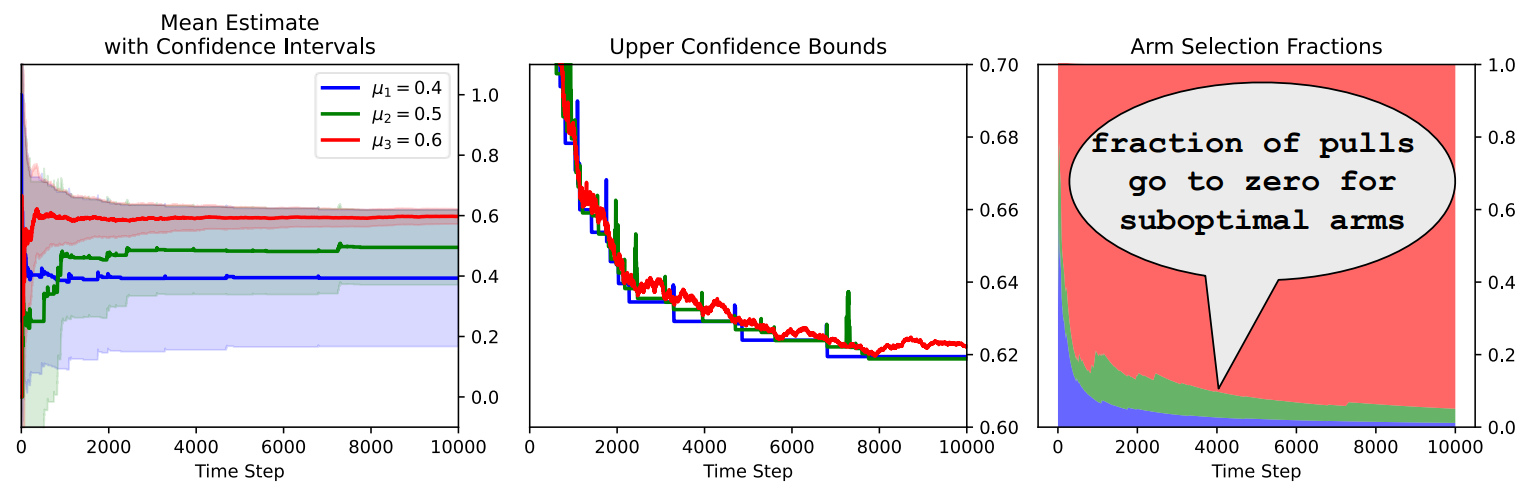
\includegraphics[width=\linewidth]{images/img_20261022_181947.png}
\end{center}

\begin{itemize}
    \item The \textbf{upper confidence bounds of the arms are nearly identical throughout}. This is a direct consequence of the algorithm: whenever one arm's UCB is the largest, that arm is pulled, its bonus shrinks and its UCB comes down towards the others. UCB thus keeps all the UCBs ``balanced''.
    \item The \textbf{worse the arm, the less often it is played}: to have the same UCB as a better arm, a worse arm (lower $\hat{\mu}_i$) needs a larger bonus, i.e.\ fewer pulls. Worse arms therefore have wider confidence intervals.
    \item The fraction of pulls $T_i(t)/t$ goes to zero for suboptimal arms (they are pulled only $O(\ln t)$ times).
\end{itemize}

\subsection{The effect of $\delta$}

Setting: two-armed Bernoulli bandit with means $[0.5 - \Delta/2,\, 0.5 + \Delta/2]$.

\begin{center}
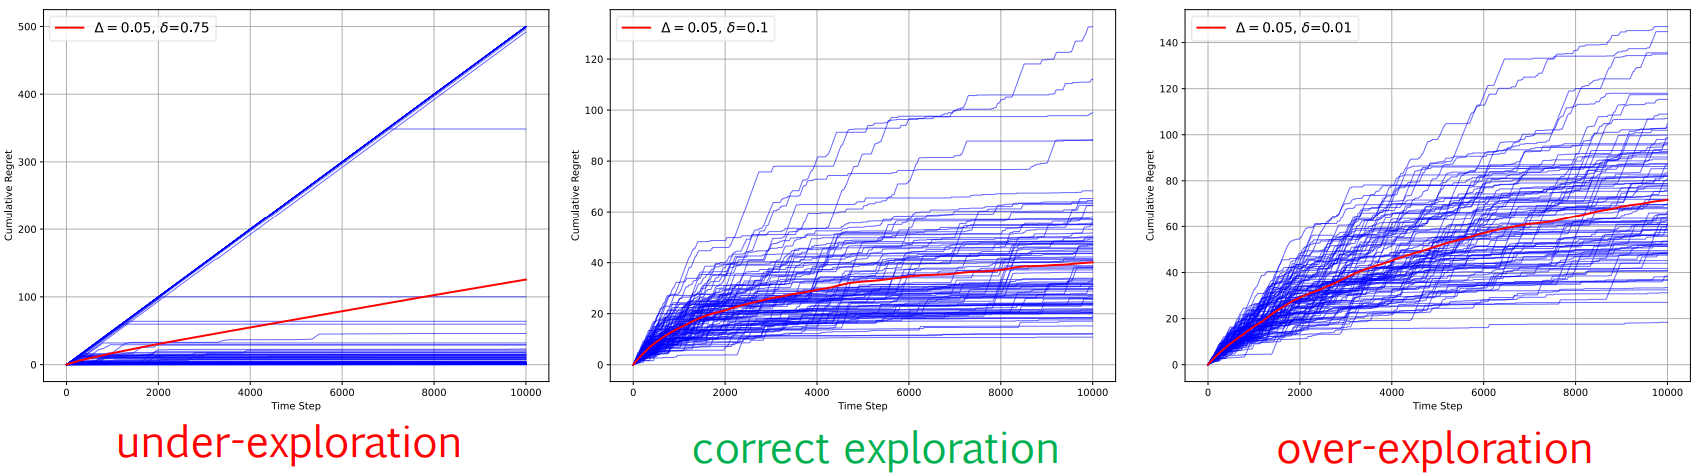
\includegraphics[width=\linewidth]{images/img_20261022_182657.png}
\end{center}

\begin{itemize}
    \item Smaller $\delta$ $\Rightarrow$ larger confidence intervals $\Rightarrow$ more exploration.
    \item \textbf{Too large $\delta$} (under-exploration): narrow intervals, so there is a real chance that the best arm gets unlucky early, its UCB drops below the mean of the other arm, and the algorithm effectively ``commits'' to the wrong arm $\Rightarrow$ large (linear) regret.
    \item \textbf{Too small $\delta$} (over-exploration): very wide intervals, the bonus dominates the empirical mean for a long time and suboptimal arms are pulled too often $\Rightarrow$ large regret.
    \item In between, correct exploration gives the smallest regret. This is the same qualitative behavior as for adaptive ETC.
\end{itemize}

\section{A problem-independent regret bound for UCB}

\subsection{Motivation}

The bound we proved,
\[
R_n \leq 3\sum_{i=1}^k \Delta_i + \sum_{i:\Delta_i > 0} \frac{16\ln n}{\Delta_i},
\]
is \textbf{problem-dependent}: it depends on the gaps of the instance. If some $\Delta_i$ is arbitrarily small, the bound blows up and becomes meaningless: it can be much larger than the trivial bound
\[
R_n = \sum_i \Delta_i\,\mathbb{E}[T_i(n)] \leq \Delta_{\max} \sum_i \mathbb{E}[T_i(n)] = n\,\Delta_{\max}, \qquad \Delta_{\max} = \max_i \Delta_i,
\]
which always holds (at most, we pay the largest gap at every round). For instance, with $\Delta_i = 10^{-6}$ and $n = 10^4$, the term $\frac{16\ln n}{\Delta_i} \approx 1.5 \cdot 10^8$, while $n\Delta_{\max} \leq 10^4$ for rewards in $[0,1]$. Yet, intuitively, an arm with a tiny gap costs almost nothing per pull: even if it is pulled at every round, it contributes at most $n\Delta_i$ to the regret. Can we get a \textbf{problem-independent} (worst-case) bound, that holds uniformly over all instances?

\begin{theorem}[Alternate (problem-independent) regret bound for UCB]
For the UCB algorithm applied to a stochastic $1$-subgaussian bandit with $k$ arms and an error tolerance $\delta = 1/n^2$, the regret satisfies
\[
R_n \leq 3\sum_{i=1}^k \Delta_i + 8\sqrt{kn\ln n}.
\]
\end{theorem}

\begin{remark}
\begin{itemize}
    \item We trade the term $\sum_{i\in[k]} 1/\Delta_i$ (times $\ln n$) for a term $\sqrt{nk}$ (times $\sqrt{\ln n}$).
    \item This bound is sublinear for \emph{every} instance, independently of the gaps: $R_n = O(\sqrt{kn\ln n})$. The term $3\sum_i \Delta_i$ does not grow with $n$ (and is at most $3k$ for rewards in $[0,1]$).
    \item The algorithm is \textbf{unchanged}: this is merely a different proof strategy. Both bounds hold simultaneously, and $R_n \leq \min(\text{both})$.
\end{itemize}
\end{remark}

\subsection{Proof}

\subsubsection*{Ingredients}

Recall the main ingredients of the previous proof:
\begin{itemize}
    \item Regret decomposition lemma: $R_n = \sum_i \Delta_i\,\mathbb{E}[T_i(n)]$.
    \item Bound derived from the concentration inequality: $\mathbb{E}[T_i(n)] \leq 3 + \frac{16\ln n}{\Delta_i^2}$.
    \item A \textbf{trivial bound}: $\mathbb{E}[T_i(n)] \leq n$ (for all arms, under all conditions). More precisely, $\sum_i T_i(n) = n$.
\end{itemize}

\textbf{When is the trivial bound tighter than the concentration bound?} When
\[
\frac{16\ln n}{\Delta_i^2} \geq n \iff \Delta_i \leq \sqrt{\frac{16\ln n}{n}}.
\]
The regret from such an arm $i$ is then at most
\[
\Delta_i\,\mathbb{E}[T_i(n)] \leq \sqrt{\frac{16\ln n}{n}} \cdot n = O\big(\sqrt{n\ln n}\big).
\]
So arms with very small gaps contribute at most $O(\sqrt{n \ln n})$ each, which suggests that the goal $R_n = O(\sqrt{nk\ln n})$ is reachable.

\subsubsection*{Refined strategy}

\begin{itemize}
    \item Split the arms into two sets, according to a threshold $\Delta > 0$ (a proof parameter, \emph{not} known or used by the algorithm):
    \begin{itemize}
        \item \textbf{nearly optimal arms}: $\Delta_i < \Delta$; use the trivial bound for these arms;
        \item \textbf{clearly suboptimal arms}: $\Delta_i \geq \Delta$; use the concentration bound for these arms.
    \end{itemize}
    \item Optimize $\Delta$ to get the best expression.
\end{itemize}

\subsubsection*{Computation}

\begin{align*}
R_n &= \sum_i \Delta_i\,\mathbb{E}[T_i(n)] = \sum_{i:\Delta_i < \Delta} \Delta_i\,\mathbb{E}[T_i(n)] + \sum_{i:\Delta_i \geq \Delta} \Delta_i\,\mathbb{E}[T_i(n)] \\
&\leq n\Delta + \sum_{i:\Delta_i \geq \Delta} \Delta_i\,\mathbb{E}[T_i(n)] && \text{since } \textstyle\sum_{i:\Delta_i<\Delta}\Delta_i \mathbb{E}[T_i(n)] \leq \Delta \sum_i \mathbb{E}[T_i(n)] = n\Delta \\
&\leq n\Delta + \sum_{i:\Delta_i \geq \Delta} \Delta_i\left(3 + \frac{16\ln n}{\Delta_i^2}\right) && \text{concentration bound} \\
&= n\Delta + \sum_{i:\Delta_i \geq \Delta} \left(3\Delta_i + \frac{16\ln n}{\Delta_i}\right) \\
&\leq \sum_i 3\Delta_i + n\Delta + \frac{16k\ln n}{\Delta} && \text{since } \tfrac{1}{\Delta_i} \leq \tfrac{1}{\Delta} \text{ and there are at most } k \text{ such arms.}
\end{align*}

\textbf{Optimizing $\Delta$.} The function $\Delta \mapsto n\Delta + \frac{16k\ln n}{\Delta}$ is minimized when its derivative $n - \frac{16k\ln n}{\Delta^2}$ vanishes, i.e.\ for
\[
\Delta = \sqrt{\frac{16k\ln n}{n}}, \qquad \text{giving} \qquad n\Delta + \frac{16k\ln n}{\Delta} = 2\sqrt{16kn\ln n} = 8\sqrt{kn\ln n}.
\]
Hence $R_n \leq \sum_i 3\Delta_i + 8\sqrt{kn\ln n}$. \hfill $\square$

\subsection{Revisiting the regret plot}

\begin{center}
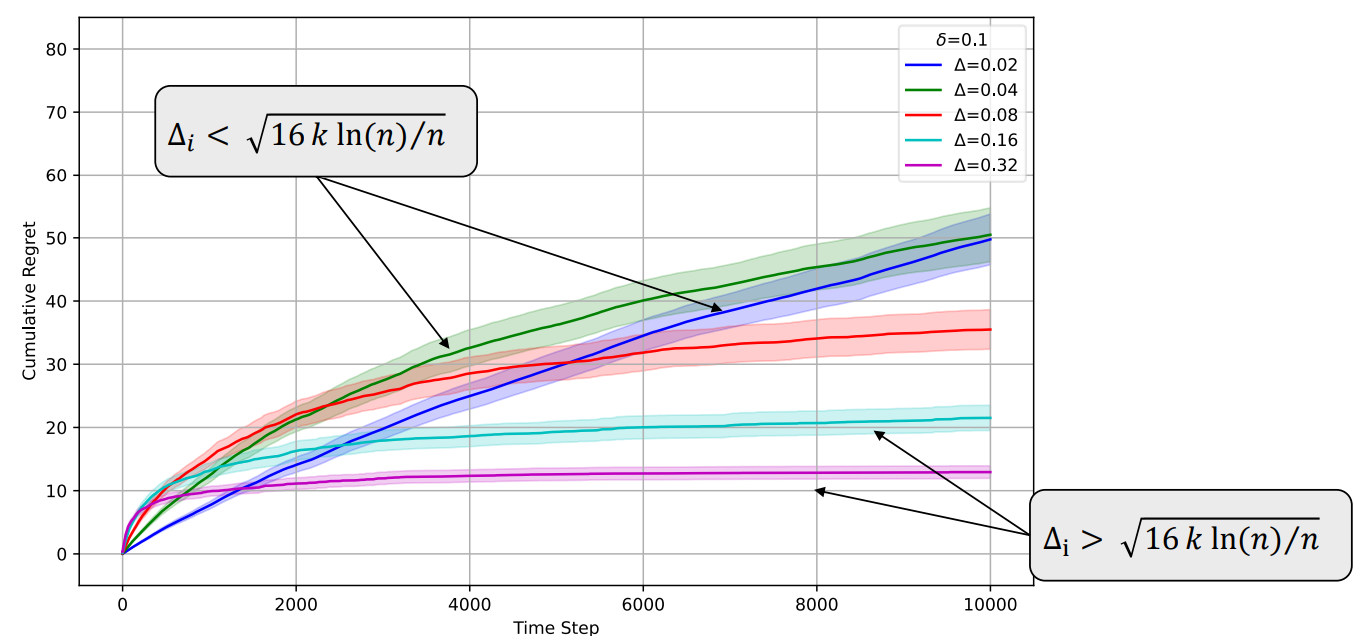
\includegraphics[width=0.8\linewidth]{images/img_20261022_185112.png}
\end{center}

\begin{itemize}
    \item It takes $O\!\left(\frac{\ln(1/\delta)}{\Delta^2}\right)$ pulls to separate two arms with gap $\Delta$ with probability $1-\delta$ (the confidence interval width $\sqrt{2\ln(1/\delta)/T}$ must become smaller than $\Delta$).
    \item $\Delta_i$ \textbf{large} ($\Delta_i > \sqrt{16k\ln n/n}$) $\Rightarrow$ confidence intervals separate early (within the horizon) $\Rightarrow$ \textbf{logarithmic} regret curves (the regime of the problem-dependent bound).
    \item $\Delta_i$ \textbf{small} ($\Delta_i < \sqrt{16k\ln n/n}$) $\Rightarrow$ separation happens late (possibly not before $n$) $\Rightarrow$ faster-growing (almost linear) regret curves, but with a small slope $\Delta_i$ (the regime of the trivial bound).
\end{itemize}

\section{Asymptotic UCB: unknown horizon}

\subsection{Motivation: why a fixed $\delta$ is not enough}

So far, the horizon $n$ was fixed a priori (and used to set $\delta = 1/n^2$). This makes sense in some applications, not in others. What happens when we do not know the horizon? Equivalently: what if we want UCB to run forever?

\begin{itemize}
    \item The main concern is that we must \textbf{eliminate any possibility of persistent error}: any error probability, however small, could lead to a large (infinite!) cumulative regret.
    \item In the current formulation, the chance of error is about the chance of the concentration event failing, which is about $\delta$.
    \begin{itemize}
        \item We cannot choose $\delta = 0$: the confidence interval would be infinite.
        \item We cannot choose a constant $\delta > 0$: there is then a small (constant) probability of getting into a bad configuration at some time $t$ (e.g.\ the best arm gets unlucky samples, its UCB drops below the mean of a suboptimal arm, and it is ignored forever) $\Rightarrow$ the regret grows linearly forever, so the expected regret is not sublinear.
    \end{itemize}
    \item In effect, we need $\delta \to 0$ over time.
    \item Consequently, we need $T_i(n) \to \infty$ for \emph{all} arms (no arm can be abandoned for good); we just control \emph{how quickly} suboptimal arms are pulled.
\end{itemize}

\subsection{Algorithm}

The fact that $\delta \to 0$ over time is reflected in the confidence intervals:
\begin{itemize}
    \item originally: $UCB_i(t, \delta) = \hat{\mu}_i(t) + \sqrt{\frac{2\ln(1/\delta)}{T_i(t)}}$;
    \item new formulation: $UCB_i(t) = \hat{\mu}_i(t) + \sqrt{\frac{8\ln t}{T_i(t)}}$.
\end{itemize}
This corresponds to choosing a time-varying confidence level $\delta_t = t^{-4}$, since $2\ln(1/\delta_t) = 2\ln(t^4) = 8\ln t$. The rest of the algorithm remains identical!

\begin{definition}\textbf{(Asymptotic UCB).}
\begin{tabbing}
\hspace{1.5em}\=\kill
\textbf{for} $t = 1, 2, \dots$ \textbf{do}: \\
\> choose $A_t = \arg\max_i \left(\hat{\mu}_i(t-1) + \sqrt{\dfrac{8\ln t}{T_i(t-1)}}\right)$ \quad (with the index $= \infty$ if $T_i(t-1) = 0$); \\
\> observe $X_t$ and update $UCB_i(t)$ for all $i$.
\end{tabbing}
\end{definition}

\begin{remark}
\begin{itemize}
    \item Now \emph{all} the UCBs must be updated at each round, not only the one of the pulled arm: the bonus depends on $t$ through $\ln t$.
    \item If an arm is not played for a long time, its confidence interval slowly grows (its $T_i$ is frozen but $\ln t$ increases). Its UCB grows (very slowly) without bound, so an arm cannot be neglected forever: each arm is pulled every so often.
    \item Hence no ``error'' (mistake in identifying the best arm) is permanent.
    \item This is \textbf{not} the same as $\delta = 1/n^2$ in the proof of last week: that $\delta$ was fixed over time (but depended on the known horizon $n$), whereas here $\delta_t$ gradually decreases with the current time $t$, and no knowledge of $n$ is needed (``anytime'' algorithm).
\end{itemize}
\end{remark}

\begin{theorem}[Regret of asymptotic UCB]
For any $1$-subgaussian bandit, the regret of the asymptotic UCB algorithm satisfies, for all $n$,
\[
R_n \leq \sum_{i:\Delta_i > 0}\left(4\Delta_i + \frac{32\ln n}{\Delta_i}\right),
\qquad\text{hence}\qquad
\limsup_{n\to\infty} \frac{R_n}{\ln n} \leq \sum_{i:\Delta_i > 0} \frac{32}{\Delta_i}.
\]
\end{theorem}

\subsection{Regret bound: proof sketch}

As in the fixed-horizon version, the key is to prove that, for every suboptimal arm $i$,
\[
\mathbb{E}[T_i(n)] \leq \frac{32\ln n}{\Delta_i^2} + 4,
\]
and the theorem then follows from the regret decomposition. We broadly follow the same steps:
\begin{itemize}
    \item Define good events such that, under the good event (``normal circumstances''), the number of pulls of a suboptimal arm is bounded by some $u_i$.
    \item Show that the probability of the bad event is small (concentration inequality).
\end{itemize}
Differences from the fixed-horizon case:
\begin{itemize}
    \item the good event now \textbf{depends on time} $t$;
    \item a careful use of the union bound (over rounds, then over the possible numbers of pulls).
\end{itemize}

As before, assume without loss of generality that arm $1$ is optimal.

\subsubsection*{Defining good events: fixed horizon versus asymptotic}

\begin{center}
\renewcommand{\arraystretch}{1.6}
\begin{tabular}{p{0.45\linewidth}|p{0.45\linewidth}}
\textbf{Fixed horizon} & \textbf{Asymptotic} \\
\hline
$G = G_1 \cap G_i$, where & $G_t = G_{1,t} \cap G_{i,t}$, where \\
$G_1 = \left\{\mu_1 < \min_{t\in[n]} \hat{\mu}_1(t) + \sqrt{\frac{2}{T_1(t)}\ln\frac{1}{\delta}}\right\}$ & $G_{1,t} = \left\{\mu_1 < \hat{\mu}_1(t) + \sqrt{\frac{8}{T_1(t)}\ln t}\right\}$ \\
$G_i = \left\{\hat{\mu}_{iu_i} + \sqrt{\frac{2}{u_i}\ln\frac{1}{\delta}} < \mu_1\right\}$ & $G_{i,t} = \left\{\mu_i > \hat{\mu}_i(t) - \sqrt{\frac{8}{T_i(t)}\ln t}\right\}$ \\
Conditional on $G$: $T_i(n) \leq \frac{8\ln(1/\delta)}{\Delta_i^2} =: u_i$. & Conditional on $G_t$: $T_i(t) \leq \frac{32\ln t}{\Delta_i^2} =: u_i(t)$ \textbf{or} arm $i$ is not pulled in round $t$.
\end{tabular}
\end{center}

Interpretation of the asymptotic good events:
\begin{itemize}
    \item $G_{1,t}$: the UCB of arm $1$ is above its true mean at time $t$;
    \item $G_{i,t}$: the LCB of arm $i$ is below its true mean at time $t$.
\end{itemize}
The fixed-horizon good event is a single event covering the whole run; the asymptotic one is a family of events, one per round, and only requires the two confidence intervals to be correct \emph{at round $t$}.

\begin{remark}[Indices]
As in the slides, we write all quantities ``at time $t$'' to lighten notation. Strictly speaking, the decision at round $t$ uses $\hat{\mu}_i(t-1)$ and $T_i(t-1)$ (with the bonus $\sqrt{8\ln t/T_i(t-1)}$); the argument is identical.
\end{remark}

\subsubsection*{Step 1: under $G_t$, a suboptimal arm with many pulls is not chosen}

We need to show
\[
G_t \cap \{A_t = i\} \Rightarrow T_i(t) \leq \frac{32\ln t}{\Delta_i^2},
\qquad\text{equivalently}\qquad
G_t \cap \left\{T_i(t) > \frac{32\ln t}{\Delta_i^2}\right\} \Rightarrow A_t \neq i.
\]
This uses elementary logic: $A \Rightarrow B \iff (B^c \Rightarrow A^c)$, and more generally $C \cap A \Rightarrow B \iff (C \cap B^c \Rightarrow A^c)$. (Also: $A \Rightarrow B \cup C \iff (A \cap B^c \Rightarrow C)$, which gives the ``$T_i(t) \leq u_i(t)$ \emph{or} arm $i$ not pulled'' form of the table.)

\begin{proof}
Assume that both $G_t$ and $T_i(t) > \frac{32\ln t}{\Delta_i^2}$ occur.
\begin{itemize}
    \item From $T_i(t) > \frac{32\ln t}{\Delta_i^2}$: $\Delta_i^2 > \frac{32\ln t}{T_i(t)} = 4\cdot\frac{8\ln t}{T_i(t)}$, so
    \[
    \Delta_i > 2\sqrt{\frac{8\ln t}{T_i(t)}}.
    \]
    \item From $G_{i,t}$ and $G_{1,t}$, using $\mu_1 = \mu_i + \Delta_i$:
    \[
    \underbrace{\hat{\mu}_i(t) - \sqrt{\frac{8\ln t}{T_i(t)}}}_{LCB_i(t)} + \Delta_i < \mu_i + \Delta_i = \mu_1 < \underbrace{\hat{\mu}_1(t) + \sqrt{\frac{8\ln t}{T_1(t)}}}_{UCB_1(t)}.
    \]
    \item Combining, since $\Delta_i > 2\sqrt{8\ln t/T_i(t)}$:
    \[
    UCB_i(t) = \hat{\mu}_i(t) + \sqrt{\frac{8\ln t}{T_i(t)}} = \hat{\mu}_i(t) - \sqrt{\frac{8\ln t}{T_i(t)}} + 2\sqrt{\frac{8\ln t}{T_i(t)}} < \hat{\mu}_i(t) - \sqrt{\frac{8\ln t}{T_i(t)}} + \Delta_i < UCB_1(t).
    \]
\end{itemize}
So $UCB_i(t) < UCB_1(t)$, and arm $i$ is not pulled in round $t$.
\end{proof}

Graphically, on the good event: $\dots < LCB_i(t) < \mu_i < \dots < \mu_1 < UCB_1(t)$, and once $T_i(t)$ is large, the interval of arm $i$ is narrower than $\Delta_i/2$ on each side, so $UCB_i(t) < \mu_1 < UCB_1(t)$.

\subsubsection*{Step 2: bounding $\mathbb{E}[T_i(n)]$}

\textbf{Fixed horizon} (recap): $\mathbb{E}[T_i(n)] \leq \mathbb{E}[\mathbb{I}\{G\}T_i(n)] + \mathbb{E}[\mathbb{I}\{G^c\}T_i(n)] \leq u_i + \mathbb{P}(G^c)\,n$, with $\mathbb{P}(G_i^c) \leq n\delta + \exp\left(-\frac{u_i c^2 \Delta_i^2}{2}\right)$; put together, this gives the desired result. This approach is \textbf{too loose for the asymptotic version} (``$n = \infty$''): the term $\mathbb{P}(G^c)\,n$ requires $\mathbb{P}(G^c) \lesssim 1/n$ for a known $n$.

\textbf{Asymptotic}: we decompose \emph{round by round}. Since $\mathbb{I}\{G_t\} + \mathbb{I}\{G_t^c\} \equiv 1$,
\begin{align*}
\mathbb{E}\big[\mathbb{I}\{A_t = i\}\big] &= \mathbb{E}\big[\mathbb{I}\{G_t\}\,\mathbb{I}\{A_t = i\}\big] + \mathbb{E}\big[\mathbb{I}\{G_t^c\}\,\mathbb{I}\{A_t = i\}\big] \\
&\leq \mathbb{E}\big[\mathbb{I}\{T_i(t) \leq u_i(t)\}\,\mathbb{I}\{A_t = i\}\big] + \mathbb{E}\big[\mathbb{I}\{G_t^c\}\big],
\end{align*}
using step 1 for the first term ($G_t \cap \{A_t = i\} \subseteq \{T_i(t) \leq u_i(t)\} \cap \{A_t = i\}$) and $\mathbb{I}\{A_t = i\} \leq 1$ for the second. Summing over rounds, and using $u_i(t) \leq u_i(n)$ for $t \leq n$:
\begin{align*}
\mathbb{E}[T_i(n)] = \sum_{t\in[n]} \mathbb{E}\big[\mathbb{I}\{A_t = i\}\big]
&\leq \sum_{t\in[n]} \mathbb{E}\big[\mathbb{I}\{T_i(t) \leq u_i(n)\}\,\mathbb{I}\{A_t = i\}\big] + \sum_{t\in[n]}\mathbb{P}(G_t^c) \\
&\leq u_i(n) + 1 + \sum_{t=1}^\infty \mathbb{P}(G_t^c) \\
&\leq \frac{32\ln n}{\Delta_i^2} + 1 + \sum_{t=1}^\infty \frac{2}{t^3} \leq \frac{32\ln n}{\Delta_i^2} + 4.
\end{align*}
Explanations:
\begin{itemize}
    \item \textbf{Counting argument}: $\sum_t \mathbb{I}\{T_i(t) \leq u_i(n)\}\,\mathbb{I}\{A_t = i\}$ counts the rounds in which arm $i$ is pulled while its counter is at most $u_i(n)$. How many times can one increment a counter while it is less than $u_i$? At most $u_i + 1$ times (each pull increments $T_i$ by one).
    \item $\mathbb{P}(G_t^c) \leq 2t^{-3}$ (shown below), and $\sum_{t=1}^\infty \frac{1}{t^3} \leq 1 + \int_1^\infty \frac{1}{t^3}\,dt = 1.5$, so $\sum_t \frac{2}{t^3} \leq 3$. Crucially, this series \textbf{converges}: the total probability of bad events over an infinite horizon is finite. This is why $\delta_t$ must decrease fast enough ($\delta_t = t^{-4}$).
\end{itemize}

\subsubsection*{Step 3: bounding $\mathbb{P}(G_t^c)$}

We need to show $\mathbb{P}(G_{1,t}^c) \leq t^{-3}$; the same bound holds for $\mathbb{P}(G_{i,t}^c)$ (by symmetry, for the lower tail). Together, by the union bound,
\[
\mathbb{P}(G_t^c) \leq \mathbb{P}(G_{1,t}^c) + \mathbb{P}(G_{i,t}^c) \leq 2t^{-3}.
\]
As in the fixed-horizon proof, $T_1(t)$ is random, so we take a union over all its possible values $s \in [t]$ (if $T_1(t) = 0$, the UCB is infinite and $G_{1,t}$ holds), and work with $\hat{\mu}_{1,s}$, the average of the first $s$ samples of arm $1$:
\[
G_{1,t}^c = \left\{\mu_1 \geq \hat{\mu}_1(t) + \sqrt{\frac{8\ln t}{T_1(t)}}\right\} \subseteq \bigcup_{s=1}^t \left\{\mu_1 \geq \hat{\mu}_{1,s} + \sqrt{\frac{8\ln t}{s}}\right\}.
\]
Then, by the union bound and the Chernoff bound (for $s$ i.i.d.\ $1$-subgaussian samples, $\mathbb{P}\big(\mu \geq \hat{\mu}_s + \sqrt{2\ln(1/\delta)/s}\big) \leq \delta$), with $\delta = t^{-4}$:
\[
\mathbb{P}(G_{1,t}^c) \leq \sum_{s=1}^t \mathbb{P}\left(\mu_1 \geq \hat{\mu}_{1,s} + \sqrt{\frac{8\ln t}{s}}\right) = \sum_{s=1}^t \mathbb{P}\left(\mu_1 \geq \hat{\mu}_{1,s} + \sqrt{\frac{2\ln(1/t^{-4})}{s}}\right) \leq \sum_{s=1}^t t^{-4} = t^{-3}.
\]

\begin{remark}[Why $t^{-4}$?]
The union over the $t$ possible values of $T_1(t)$ costs a factor $t$, so the per-$s$ error probability $\delta_t$ must satisfy that $\sum_t t\,\delta_t$ converges. With $\delta_t = t^{-4}$, we get $\sum_t 2t^{-3} < \infty$. (A choice like $\delta_t = t^{-2}$ would give $\sum_t t^{-1} = \infty$, which is not enough for this proof.)
\end{remark}

\subsubsection*{Conclusion}

Multiplying by $\Delta_i$ and summing over suboptimal arms gives $R_n \leq \sum_{i:\Delta_i>0}\left(4\Delta_i + \frac{32\ln n}{\Delta_i}\right)$. Dividing by $\ln n$ and letting $n \to \infty$:
\[
\limsup_{n\to\infty} \frac{R_n}{\ln n} \leq \sum_{i:\Delta_i > 0} \frac{32}{\Delta_i}.
\]
This is the \textbf{same order} as the result of last week ($\ln n/\Delta_i$), but now we \textbf{do not need to know $n$ a priori}! The price is only a worse constant ($32$ instead of $16$).

\subsection{Asymptotically optimal UCB}

The constant can be squeezed further. Algorithm 6 and Theorem 8.1 in Lattimore \& Szepesvári give an asymptotically optimal result:
\[
\limsup_{n\to\infty} \frac{R_n}{\ln n} \leq \sum_{i:\Delta_i > 0} \frac{2}{\Delta_i}.
\]
Differences with our version:
\begin{itemize}
    \item the exploration bonus is $\sqrt{\frac{2\ln f(t)}{T_i(t-1)}}$ with $f(t) = 1 + t\ln^2(t)$, instead of $f(t) = t^4$ (i.e.\ $\sqrt{8\ln t/T_i(t-1)}$): a much smaller bonus, hence less exploration;
    \item the good events measure the UCB crossing the threshold $\mu_1 - \varepsilon$ rather than $\mu_1$ (a finer analysis).
\end{itemize}
``Asymptotically optimal'' means that no reasonable algorithm can have a better constant: this matches the lower bound of Lai and Robbins (see below), which we do not study in this course.

\subsection{UCB: a long history}

\begin{itemize}
    \item \textbf{1985}: Lai and Robbins give a clean formulation of the multi-armed bandit problem.
    \begin{itemize}
        \item They proved the fundamental \textbf{logarithmic lower bound} (we do not study lower bounds; they serve to understand the best possible performance of any algorithm).
        \item They also introduced the idea of \textbf{optimism} and of using confidence bounds.
    \end{itemize}
    \item \textbf{1985--1995}: UCB algorithm proposed, asymptotic regret bounds.
    \item \textbf{2002}: Auer et al.\ proposed the \textbf{UCB1} algorithm and analysed its (finite-time) regret. This is what we saw in class.
    \item \textbf{2010--2017}: asymptotically optimal and minimax-optimal algorithms: MOSS, KL-UCB, etc.
    \item Coming up: Thompson Sampling, an algorithm from \textbf{1933}!
\end{itemize}

\section{Thompson Sampling}

\subsection{Prelude: Bayesian statistics}

In Bayesian statistics, we maintain a \textbf{belief distribution} over unknown quantities.
\begin{itemize}
    \item The belief distribution measures all we know about the unknown.
    \item Without any data, the belief distribution has a large variance.
    \item With more data, the belief distribution concentrates around the true parameter.
\end{itemize}
Formally, the belief is updated with Bayes' rule: starting from a \textbf{prior} $f_0(\mu)$, after observing data $D$ we get the \textbf{posterior}
\[
f(\mu \mid D) = \frac{\mathbb{P}(D \mid \mu)\, f_0(\mu)}{\int \mathbb{P}(D \mid \mu')\, f_0(\mu')\,d\mu'} \propto \mathbb{P}(D \mid \mu)\, f_0(\mu).
\]

\begin{center}
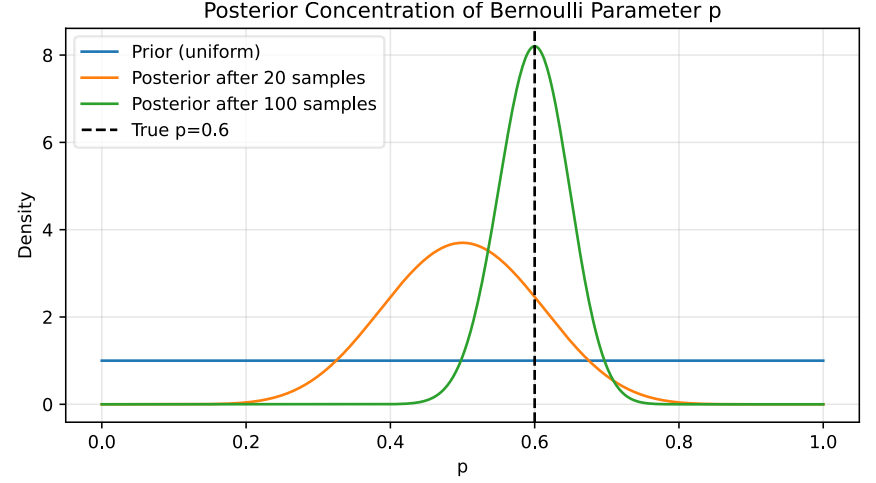
\includegraphics[width=0.707\linewidth]{images/img_20261022_201339.png}
\end{center}

\subsection{Bayesian view of bandits}

\begin{itemize}
    \item In multi-armed bandits with $\{0,1\}$ rewards, the unknown variables are the mean rewards of each arm: $\mu_1, \mu_2, \dots, \mu_k$.
    \item We maintain a belief $f_{i,t}(\mu)$ for all arms $i$, at all times $t$, instead of $\hat{\mu}_i$ and a UCB.
    \item Initially, we know nothing about $\mu_i$: any value in $[0,1]$ is equally likely. The \textbf{prior} belief $f_{i,0}(\mu)$ for each arm $i$ is the uniform distribution on $[0,1]$.
    \item Over time, we pull arms and observe rewards, and the belief $f_{i,t}(\cdot)$ concentrates near $\mu_i$.
\end{itemize}

\begin{center}
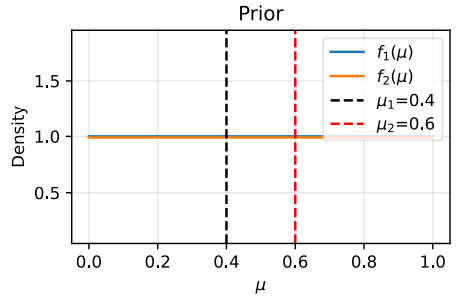
\includegraphics[width=0.32\linewidth]{images/img_20261022_203209.png}
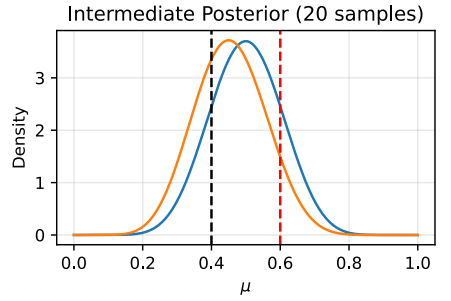
\includegraphics[width=0.32\linewidth]{images/img_20261022_203131.png}
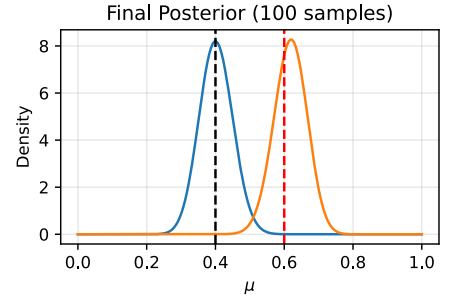
\includegraphics[width=0.32\linewidth]{images/img_20261022_203143.png}
\end{center}

\subsection{Algorithm}

Thompson Sampling is a \textbf{randomized} algorithm for multi-armed bandits.
\begin{itemize}
    \item The algorithm maintains a belief distribution over the possible arm values at all times. Contrast: UCB maintains a point estimate and a confidence interval of the arm values.
    \item At each step, the algorithm:
    \begin{itemize}
        \item samples values $\tilde{\mu}_1, \tilde{\mu}_2, \dots, \tilde{\mu}_k$ according to the belief distributions;
        \item plays the arm with the highest sampled value (a form of optimism);
        \item observes the data and updates the belief of the played arm.
    \end{itemize}
\end{itemize}

\begin{center}
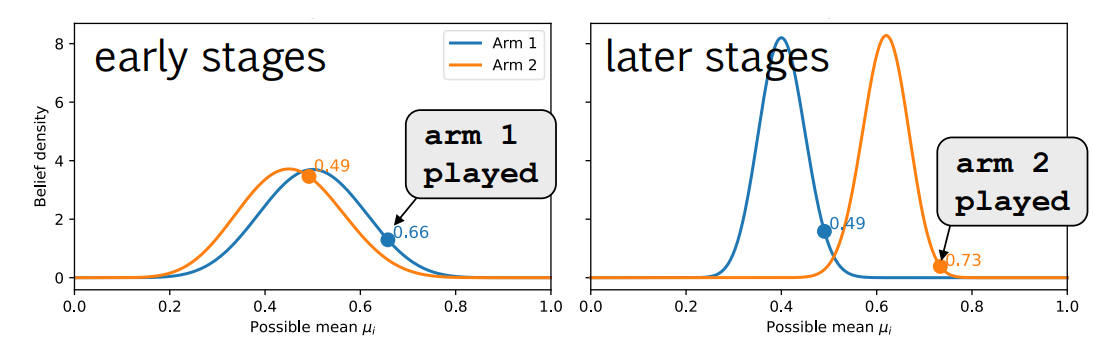
\includegraphics[width=0.8\linewidth]{images/img_20261022_203241.png}
\end{center}

\begin{definition}\textbf{(Thompson Sampling).}
\begin{tabbing}
\hspace{1.5em}\=\hspace{1.5em}\=\kill
\textbf{for} $t = 1, 2, \dots$ \textbf{do}: \\
\> \textbf{for} $i = 1, 2, \dots, k$ \textbf{do}: sample $\tilde{\mu}_i(t) \sim f_{i,t}(\cdot)$; \\
\> choose $A_t = \arg\max_i \tilde{\mu}_i(t)$; \\
\> observe $X_t$, update $f_{A_t, t}(\cdot)$.
\end{tabbing}
\end{definition}

\subsection{Intuition}

\begin{itemize}
    \item Exploration happens through the \textbf{randomness in the sampling}.
    \item Initially, beliefs are weak $\Rightarrow$ larger variance $\Rightarrow$ samples are spread out, any arm can come out on top $\Rightarrow$ more exploration.
    \item Over time, beliefs concentrate, samples are close to the true means $\Rightarrow$ the arm with the highest mean almost always wins $\Rightarrow$ exploitation.
    \item Smooth transition from exploration to exploitation, and the beliefs of the candidates for best arm concentrate more quickly (they are sampled more).
    \item Equivalently, Thompson Sampling plays each arm with the (posterior) \emph{probability that it is the best arm}: an arm that is clearly worse has a tiny probability of producing the largest sample, so it is rarely played.
\end{itemize}

\subsubsection*{Evolution of the posterior}

\begin{center}
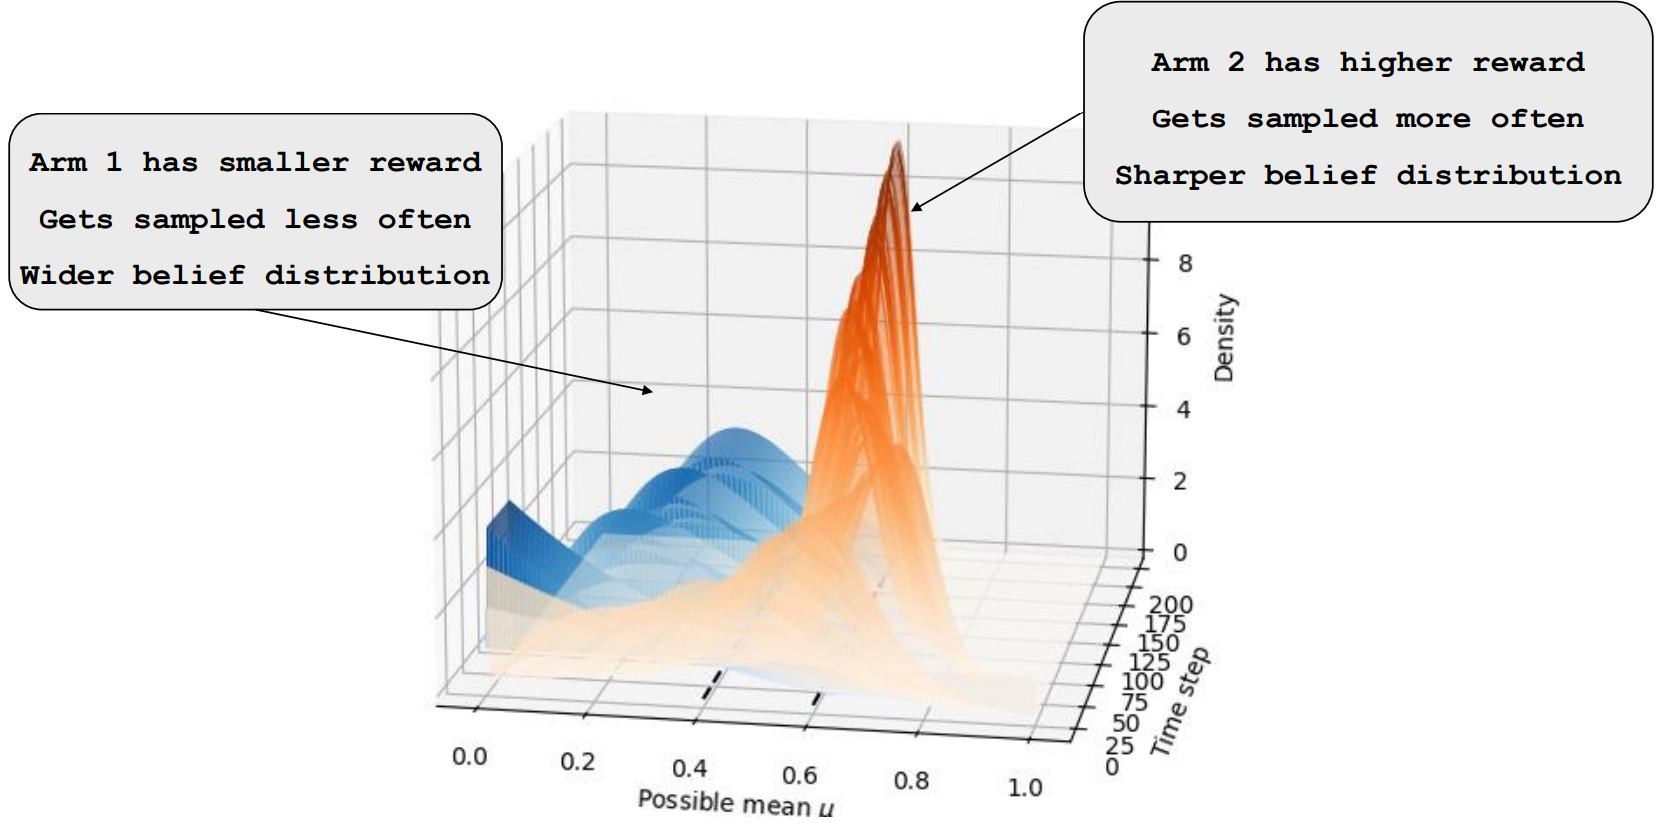
\includegraphics[width=0.8\linewidth]{images/img_20261022_204105.png}
\end{center}

This is the Bayesian analogue of what we observed for UCB: worse arms have wider confidence intervals.

\subsubsection*{Thompson Sampling versus UCB}

Setting: two-armed Bernoulli bandit with means $[0.4, 0.6]$.

\begin{center}
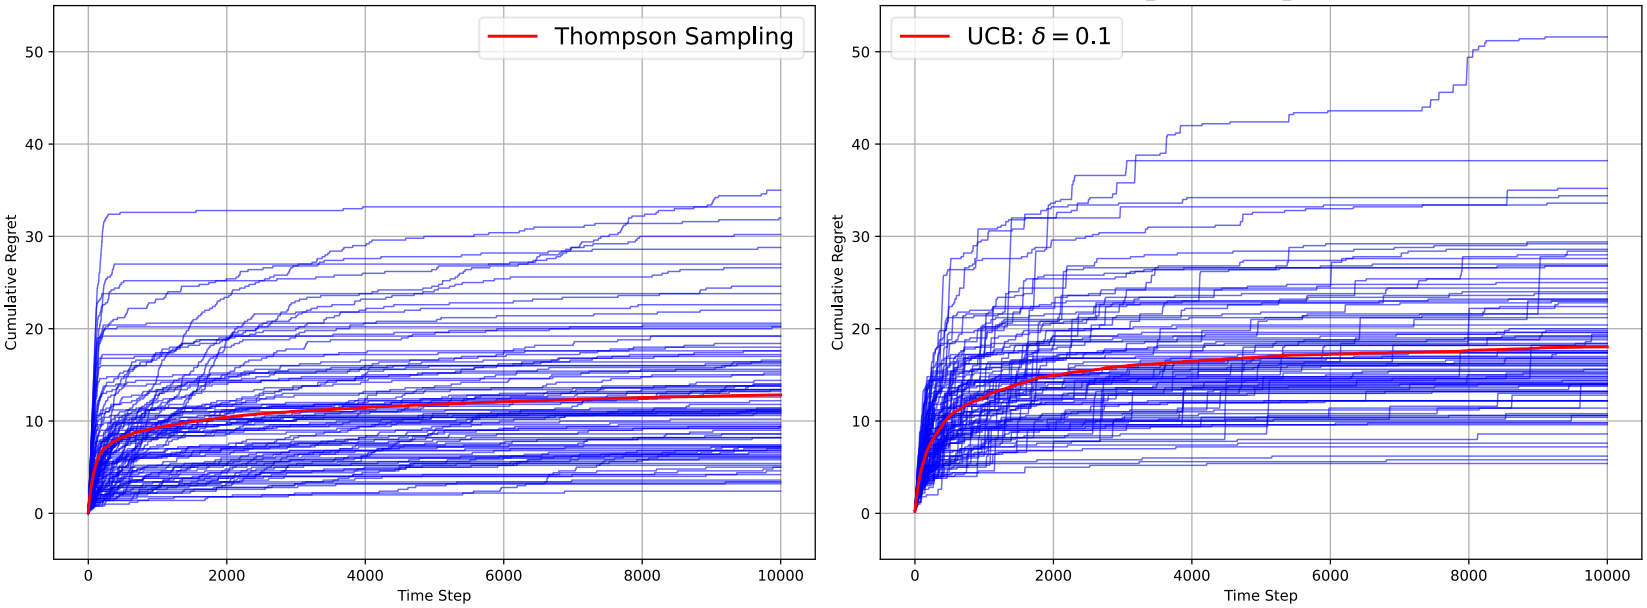
\includegraphics[width=\linewidth]{images/img_20261022_204249.png}
\end{center}

\begin{itemize}
    \item The regret curves of Thompson Sampling are similar to those of UCB.
    \item Smooth exploration-exploitation tradeoff.
    \item In practice, Thompson Sampling can be better than UCB.
\end{itemize}

\subsection{Calculating posteriors: Beta-Bernoulli}

In the Bernoulli bandit setting (rewards $0$ or $1$), we use a convenient \textbf{conjugate prior}: the \textbf{Beta distribution}.

\begin{definition}[Beta distribution]
The Beta distribution with parameters $\alpha, \beta > 0$ has density on $[0,1]$
\[
f(x) = \frac{x^{\alpha - 1}(1-x)^{\beta - 1}}{B(\alpha, \beta)}, \qquad B(\alpha, \beta) = \frac{\Gamma(\alpha)\Gamma(\beta)}{\Gamma(\alpha + \beta)}.
\]
Its mean is $\frac{\alpha}{\alpha + \beta}$, and its variance $\frac{\alpha\beta}{(\alpha+\beta)^2(\alpha+\beta+1)}$ decreases as $\alpha + \beta$ grows. $\text{Beta}(1,1)$ is the uniform distribution on $[0,1]$.
\end{definition}

\begin{itemize}
    \item Belief for arm $i$: $\mu_i \sim \text{Beta}(\alpha_i, \beta_i)$, where $\alpha_i$ counts the past successes and $\beta_i$ the past failures (starting from $\alpha_i = \beta_i = 1$ for the uniform prior, so $\alpha_i - 1$ successes and $\beta_i - 1$ failures have been observed).
    \item After observing a reward $r_t \in \{0, 1\}$ from arm $i$:
    \[
    \alpha_i \leftarrow \alpha_i + r_t, \qquad \beta_i \leftarrow \beta_i + (1 - r_t).
    \]
    \item The posterior remains a Beta distribution (this is what \emph{conjugate} means): updating beliefs just amounts to incrementing these two counters.
    \item More data $\Rightarrow$ the posterior becomes narrower (more confident).
    \item Successes ($1$) shift the density rightward; failures ($0$) shift it leftward.
\end{itemize}

\begin{remark}[Why the posterior stays Beta]
With a $\text{Beta}(\alpha,\beta)$ prior and one Bernoulli observation $r \in \{0,1\}$ (likelihood $\mu^r(1-\mu)^{1-r}$), Bayes' rule gives
\[
f(\mu \mid r) \propto \mu^r(1-\mu)^{1-r} \cdot \mu^{\alpha-1}(1-\mu)^{\beta-1} = \mu^{(\alpha + r) - 1}(1-\mu)^{(\beta + 1 - r) - 1},
\]
which is the (unnormalized) density of $\text{Beta}(\alpha + r, \beta + 1 - r)$.
\end{remark}

\begin{remark}[Example]
Arm $i$ with a uniform prior, pulled $5$ times with rewards $1, 0, 1, 1, 0$: the posterior is $\text{Beta}(1 + 3, 1 + 2) = \text{Beta}(4, 3)$, with mean $4/7$. Thompson Sampling draws $\tilde{\mu}_i \sim \text{Beta}(4,3)$, compares it with the samples of the other arms, and plays the arm with the largest sample.
\end{remark}

\subsection{Some practical points}

\begin{itemize}
    \item Thompson Sampling has similar theoretical regret guarantees as UCB.
    \item In practice, it can sometimes achieve lower regret than UCB; it is usually competitive in performance. Benefits are seen more often in linear bandits (next lecture).
    \item Computing the posterior can be hard without conjugate priors! There are many techniques to sample from an un-normalized distribution (e.g.\ MCMC), and other techniques to approximate the posterior distribution.
    \item There is no hyperparameter to adjust the exploration-exploitation tradeoff (unlike $\delta$ in UCB). In practice, one can still:
    \begin{itemize}
        \item speed up or slow down the update of the posterior;
        \item or artificially inflate or reduce the variance of the belief distribution (more variance $\Rightarrow$ more exploration).
    \end{itemize}
    \item Thompson Sampling, like UCB, is a method to minimize regret in bandits. But what if we are only interested in identifying the best arm?
\end{itemize}

\section{Best-arm identification}

\subsection{Motivation}

Suppose a company wants to test the efficacy of drugs on mice.
\begin{itemize}
    \item There are a few different drug variants: these are the arms.
    \item We do not care about the outcome of the drug on the mice during the trial (no regret\dots{} poor mouse!).
    \item The only goal is to identify the best drug with high probability at the end of the trial.
\end{itemize}
How should the drugs be tried? (Source: Lattimore \& Szepesvári, Chapter 33.)

\subsection{Formulations}

\begin{itemize}
    \item \textbf{Basic formulation}: after $n$ rounds of playing a multi-armed bandit, identify the best arm with high probability, i.e.\ return an arm $i$ so as to minimize $\mathbb{P}(\mu^* - \mu_i > 0)$ (fixed-budget setting).
    \item \textbf{Slightly weaker requirement (PAC: probably approximately correct)}: return an arm $i$ such that $\mathbb{P}(\mu^* - \mu_i > \epsilon) \leq \delta$. We allow an $\epsilon$-suboptimal arm (``approximately correct''), with probability at least $1 - \delta$ (``probably'').
    \item \textbf{Yet another alternative}: minimize the \textbf{simple regret} at time $n+1$, $\mathbb{E}[\mu^* - \mu_i]$ where $i$ is the returned arm. This is different from cumulative regret minimization: only the quality of the final recommendation counts, not the rewards collected along the way.
\end{itemize}

\subsection{Intuition: why is this different from regret minimization?}

\begin{itemize}
    \item Regret-minimizing algorithms play suboptimal arms only $O(\log n)$ times, with confidence intervals chosen such that the error probability is $\delta = O(n^{-2})$. Spending so few samples on suboptimal arms is good for regret, but not for distinguishing them precisely from the best arm.
    \item In best-arm identification, there is \textbf{no exploration-exploitation tradeoff}: it is \textbf{pure exploration}. Pulling a bad arm costs nothing in itself, so we pull suboptimal arms more often than in regret minimization.
\end{itemize}

\subsubsection*{Baseline: uniform exploration}

Each arm is pulled $n/k$ times, and we return the empirically best arm after round $n$. Assume arm $1$ is the unique best arm. Using the union bound and then the Chernoff bound:
\[
\mathbb{P}(\mu^* - \mu_{\hat{i}} > 0) \leq \sum_{i:\Delta_i > 0} \mathbb{P}(\hat{\mu}_i \geq \hat{\mu}_1) \leq \sum_{i:\Delta_i > 0} \exp\left(-\frac{(n/k)\Delta_i^2}{4}\right),
\]
where $\hat{i}$ is the returned arm. Indeed, $(\hat{\mu}_i - \hat{\mu}_1) - (\mu_i - \mu_1)$ is the difference of two independent averages of $n/k$ samples, hence $\sqrt{2k/n}$-subgaussian, so $\mathbb{P}(\hat{\mu}_i - \hat{\mu}_1 \geq 0) = \mathbb{P}\big((\hat{\mu}_i - \hat{\mu}_1) - (\mu_i - \mu_1) \geq \Delta_i\big) \leq \exp\left(-\frac{\Delta_i^2}{2 \cdot 2k/n}\right)$.

\textbf{Can we do better?} Yes! There is no explore-exploit tradeoff, but there is still a benefit in \textbf{adaptively sampling some arms more than others}, based on the information collected so far: clearly bad arms can be discarded early, and the remaining budget spent on the hard comparisons between the top arms.

\subsection{Sequential halving}

\begin{definition}\textbf{(Sequential Halving for best-arm identification).}
Input: number of arms $k$, time horizon (budget) $n$.
\begin{tabbing}
\hspace{1.5em}\=\kill
Set the number of phases $L = \lceil \log_2 k \rceil$, active set $\mathcal{A}_1 = [k]$. \\
\textbf{for} $\ell = 1, 2, \dots, L$ \textbf{do}: \\
\> let $T_\ell = \left\lfloor \dfrac{n}{L\,|\mathcal{A}_\ell|} \right\rfloor$; \\
\> play each arm in $\mathcal{A}_\ell$ exactly $T_\ell$ times; \\
\> for each arm $i \in \mathcal{A}_\ell$, compute $\hat{\mu}_i^\ell$: the empirical mean of its last $T_\ell$ samples; \\
\> $\mathcal{A}_{\ell+1} \leftarrow$ the top $\lceil |\mathcal{A}_\ell|/2 \rceil$ arms in $\mathcal{A}_\ell$ (according to $\hat{\mu}_i^\ell$). \\
\textbf{return} the (single) arm in $\mathcal{A}_{L+1}$.
\end{tabbing}
\end{definition}

\begin{remark}
\begin{itemize}
    \item It \textbf{eliminates the worst half of the arms in each phase}, which makes a more efficient use of the experiment budget.
    \item Each phase uses (at most) the same budget $n/L$, shared among fewer and fewer arms: $T_\ell$ \textbf{increases exponentially} in $\ell$ (it roughly doubles each phase). The arms that survive the longest (the best ones) get the most samples, i.e.\ the most precise estimates, which is exactly where precision is needed.
    \item In each phase, only the samples of that phase are used (``last $T_\ell$ samples''): this keeps the samples of different phases independent, which simplifies the analysis.
    \item Compare with sequential elimination (lecture 4): both remove arms progressively, but sequential halving uses a fixed schedule (fixed budget, one halving per phase) rather than confidence intervals.
\end{itemize}
\end{remark}

\subsection{Performance of sequential halving}

\begin{theorem}[Sequential halving]
The sequential halving algorithm, applied to a stochastic $1$-subgaussian bandit with $k$ arms with mean vector $\mu_1 > \mu_2 \geq \dots \geq \mu_k$ (arms sorted by decreasing mean) for $n$ rounds, returns a suboptimal arm with probability at most
\[
3\log_2(k)\exp\left(-\frac{n}{16\,H_2(\mu)\log_2 k}\right), \qquad H_2(\mu) = \max_{j:\Delta_j > 0} \frac{j}{\Delta_j^2}.
\]
\end{theorem}

\begin{remark}[Interpretation of $H_2$]
$H_2(\mu)$ measures the \textbf{difficulty} of the instance. The term $j/\Delta_j^2$ is large when there are many arms ($j$ arms at least as good as arm $j$) with small gaps. The error probability decays exponentially in $n/(H_2 \log_2 k)$: a budget of order $H_2(\mu)\log k$ samples suffices to identify the best arm with high probability.
\end{remark}

\subsubsection*{Case 1: all suboptimal arms have the same gap}

$\mu_1 = 1$, $\mu_2 = \mu_3 = \dots = \mu_k = 1 - \Delta$ $\Rightarrow$ $H_2(\mu) = \max_j j/\Delta^2 = k/\Delta^2$.
\begin{itemize}
    \item Error rate (exponent) for sequential halving: $\sim \frac{n\Delta^2}{k\log k}$.
    \item Uniform exploration is marginally better: exponent $\sim \frac{n\Delta^2}{k}$.
\end{itemize}
Here no arm can be discarded more easily than the others, so adaptivity does not help (and costs a $\log k$ factor).

\subsubsection*{Case 2: one arm is slightly worse, all others far worse}

$\mu_1 = 1$, $\mu_2 = 1 - \Delta$, $\mu_3 = \dots = \mu_k = 0$ $\Rightarrow$ $H_2(\mu) = \max\big(2/\Delta^2, \max_{j\geq 3} j\big) = 2/\Delta^2$ (for small $\Delta$).
\begin{itemize}
    \item Error rate for sequential halving: $\sim \frac{n\Delta^2}{\log k}$.
    \item Uniform exploration: the hard comparison between arms $1$ and $2$ only gets $n/k$ samples per arm, so its exponent is $\sim \frac{n\Delta^2}{k}$.
    \item Sequential halving is \textbf{much better than uniform exploration, especially for large $k$}: it devotes more samples to deciding between arms $1$ and $2$, after quickly discarding the obviously bad arms.
\end{itemize}

\section{Summary}

\begin{itemize}
    \item \textbf{Alternate regret bound for UCB}: $R_n \leq 3\sum_i \Delta_i + 8\sqrt{kn\ln n}$, i.e.\ $O(\sqrt{n})$ up to logarithmic factors, independently of the gaps. Proof: do not use the concentration inequality for arms with small gaps ($\Delta_i < \Delta$, use $\sum_i T_i(n) = n$ instead), use it for the others, then optimize the threshold $\Delta = \sqrt{16k\ln n/n}$. The algorithm is unchanged.
    \item \textbf{Role of $\delta$ in UCB}: too large $\Rightarrow$ risk of ``committing'' to a wrong arm; too small $\Rightarrow$ over-exploration. UCB keeps the UCBs of all arms nearly equal, and worse arms are played less often.
    \item \textbf{Asymptotic UCB} (L\&S Chapter 8): unknown $n$, run forever. Index $\hat{\mu}_i(t-1) + \sqrt{8\ln t/T_i(t-1)}$ (i.e.\ $\delta_t = t^{-4}$): confidence intervals grow with time when an arm is not pulled, so the chance of a permanent error goes to zero. Similar regret result and proof as last time: $R_n \leq \sum_{i:\Delta_i>0}\left(4\Delta_i + \frac{32\ln n}{\Delta_i}\right)$, but now we do not need to know $n$. Proof: time-dependent good events $G_t$, round-by-round decomposition, counting argument, $\mathbb{P}(G_t^c) \leq 2t^{-3}$ (summable). Optimal constant: $2/\Delta_i$ (Lai--Robbins).
    \item \textbf{Thompson Sampling} (L\&S Chapter 36): Bayesian perspective, randomized algorithm. Maintain a posterior per arm (Beta$(\alpha_i, \beta_i)$ for Bernoulli rewards, updated by counting successes and failures), sample from each posterior, play the arm with the largest sample. Exploration comes from the randomness of the samples; similar guarantees as UCB, can be better in practice, no exploration hyperparameter.
    \item \textbf{Best-arm identification} (L\&S Chapter 33): a pure exploration problem (fixed budget, PAC, or simple regret formulations). Suboptimal arms are pulled more often than in regret minimization. Uniform exploration has error $\leq \sum_i \exp(-n\Delta_i^2/(4k))$; \textbf{sequential halving} halves the active set in each of $\lceil\log_2 k\rceil$ phases and has error $\leq 3\log_2 k\,\exp\big(-n/(16H_2\log_2 k)\big)$, much better when only a few arms are competitive.
\end{itemize}
